\chapter{Introdução}
\label{cha:introducao}
% \todo[inline]{Adicionar um parágrafo para explicar o que é HPC.}

Durante muito tempo, os avanços tecnológicos possibilitavam aumentar o
desempenho de semicondutores e das arquiteturas por meio do aumento da
frequência. Contudo, com o aumento da frequência, ocorre um maior consumo de
energia e, consequentemente, a temperatura do \textit{chip} aumenta. Desta
forma, as indústrias começaram a investir em outros meios para aumentar o
desempenho de arquiteturas, um exemplo, são os processadores \textit{manycore}.

Arquiteturas utilizadas na área de \hpc empregam processadores \textit{manycore} para atingir um
processamento de uma imensa quantidade de dados ou para aplicações que precisam
de um grande quantidade de tempo para serem executadas. Supercomputadores e
\textit{clusters} de computadores são utilizados para tornar a computação de
aplicações ou dados tratável do ponto de vista computacional. Essas arquiteturas
são utilizadas em aplicações científicas ou, mais atualmente, em áreas de Banco
de Dados, devido à problemas com \textit{Big Data}. Normalmente, arquiteturas
\hpc são compostas por processadores do tipo \cpu{} e aceleradores, tais como \gpu.
Atualmente, os núcleos (\textit{cores}) de arquiteturas \textit{manycore}
aumentam continuamente. A Figura~\ref{fig:graphCores} mostra o número total de
\textit{cores} do supercomputador em primeiro lugar no \textit{ranking} do
TOP500\footnote{\url{http://top500.org}}, confirmando esse comportamento.
% \todo[inline]{Adicionar comentário sobre imagem de \textit{cores}}

% \todo[inline]{Saiu a lista de novembro. Atualizar o gráfico.}

\begin{figure}[t]
	\centering
	\caption{Crescimento do número de núcleos do supercomputadores número 1 do \textit{ranking} Top500 (dados extraídos do Top500).}
	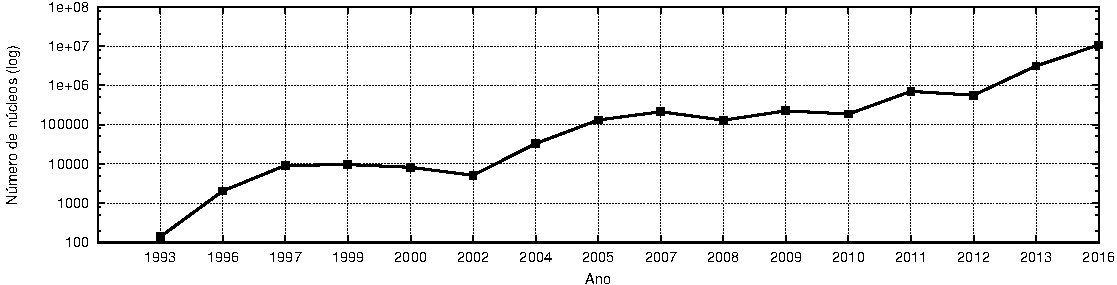
\includegraphics[width=\textwidth]{figs/top500.pdf}
    \caption*{Fonte: desenvolvido pelo autor.}
	\label{fig:graphCores}
\end{figure}

% \todo[inline]{Saiu a lista de novembro. Atualizar o gráfico e o texto.}

\begin{figure}[t]
	\centering
	\caption{Eficiência energética do supercomputador número 1 do \textit{ranking} Green500 (dados extraídos do Green500).}
        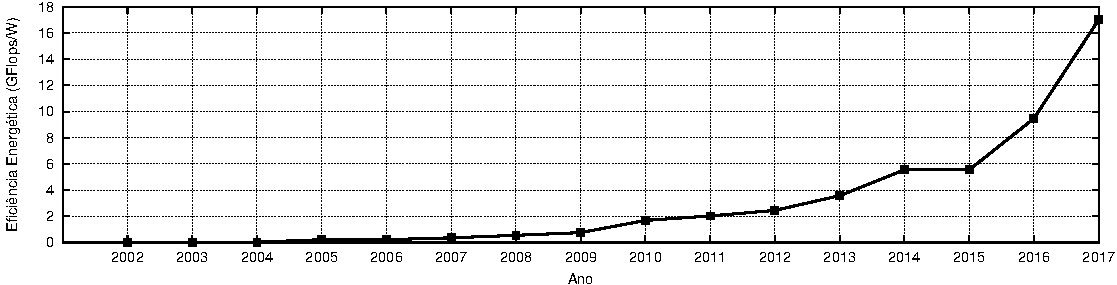
\includegraphics[width=\textwidth]{figs/green500.pdf}
    \caption*{Fonte: desenvolvido pelo autor.}
	\label{fig:graphEnergy}
\end{figure}


Até a última década, o desempenho das arquiteturas utilizadas em \hpc era quantificado quase
que exclusivamente pelo seu poder de processamento, usualmente medido por
\flops. Contudo, o consumo excessivo de energia é uma barreira para o aumento de
desempenho de forma escalável nestas plataformas.
Essa preocupação com o aumento de energia é ressaltada pelo relatório emitido
pelo Departamento de Defesa do Governo dos Estados Unidos (DARPA/IPTO)
~\cite{Kogge2008}. O relatório ressalta que a potência máxima aceitável para supercomputadores
\textit{Exascale} (10$^{18}$) seria de 20 MW, isto é, com
essas características, um supercomputador deveria possuir uma eficiência energética de 50 GFlops/W.
Por outro lado, atualmente, os supercomputadores mais energicamente eficientes
possuem uma eficiência energética de no máximo $17$ GFlops/W, como pode ser observado nos dados extraídos do \textit{ranking}
Green500\footnote{\url{https://www.top500.org/green500/}} mostrados na Figura~\ref{fig:graphEnergy}.
Este valor é quase 3 vezes menor que o ressaltado pelo
relatório da DARPA/IPTO, sendo assim, atualmente a eficiência energética de
supercomputadores está ainda distante da ideal. Portanto, para que
supercomputadores tenham potencial para atingir o \textit{Exascale} é necessário
um consumo energético viável e um alto desempenho. Contudo, o crescimento dessas
duas variáveis não é proporcional.


Por essa razão, o estudo de técnicas que melhorem a eficiência energética em
plataformas \hpc está se tornando muito importante.  Recentemente, uma nova
classe de processadores \textit{manycore} de baixa potência tais como o Sunway
SW26010~\cite{sunway:2016}, Mellanox TILE-Gx~\cite{Valero:2012} e Kalray
\mppa~\cite{Castro-IA3:2013} foram desenvolvidos. Esses processadores possuem
centenas de núcleos de processamento capazes de lidar com paralelismo de dados e
tarefas com baixo consumo de energia.

Apesar desses processadores \textit{manycore} fornecerem uma melhor eficiência
energética~\cite{Castro-IA3-JPDC:2014}, eles possuem uma arquitetura particular
que torna o desenvolvimento de aplicações paralelas uma tarefa
desafiadora~\cite{Varghese14,Castro-PARCO:2016,Castro-SBAC-PAD:2014}. Núcleos de
processamento sem coerência de \textit{cache} são, geralmente, distribuídos em
uma arquitetura organizada em \textit{clusters}, onde cada \textit{cluster}
possui uma memória local (compartilhada somente entre os núcleos do
\textit{cluster}). Dessa forma, a comunicação entre \textit{clusters} deve que
ser efetuada através de uma \noc de maneira distribuída.
Por essa razão, o tempo de comunicação pode variar entre os núcleos que estão se
comunicando.
%Explicar as dificuldades.

O \mppa possui 256 núcleos distribuídos em 16 \textit{clusters}, denominados
\pes, e 4 subsistemas de \io. O ambiente do \mppa é heterogêneo, sendo utilizado
entre os \textit{clusters} e \io, uma comunicação via \noc, e
dentro de cada \textit{cluster} são utilizados comunicações diretas entre
\pes, por meio de memória compartilhada. As principais dificuldades do
desenvolvimento de aplicações para o \mppa são resumidas a seguir:

\begin{itemize}
	\item \textbf{Modelo de programação híbrido}: problema citado anteriormente, onde \textit{threads}
em um mesmo \textit{cluster} se comunicam através de memória compartilhada
local, porém a comunicação entre \textit{clusters} é feita explicitamente via
NoC, seguindo um modelo de computação distribuída; 
	\item \textbf{Comunicação explícita}: é necessária a utilização de uma \api
específica para a comunicação via NoC, similar ao POSIX de baixo nível para
\ipc; 
	\item \textbf{Memória limitada}: cada \textit{cluster} possui apenas 2MB de memória
local de baixa latência, portanto aplicações reais precisam constantemente
realizar comunicações com o subsistema de E/S;
	\item \textbf{Ausência de coerência de \textit{cache}}: cada PE possui uma memória \textit{cache} privada e sem coerência
com as \textit{caches} dos demais PEs, sendo necessário atualizar a \textit{cache} manualmente.
\end{itemize}

Uma possível solução para os problemas apresentados anteriormente é a utilização de padrões
paralelos ou \textit{skeletons}~\cite{cole-skeleton:2004}. \textit{Skeletons}
são modelos de programação paralela de alto nível de abstração. Esses modelos fornecem
vantagens para o desenvolvedor, escondendo a complexidade de aplicações
paralelas e distribuídas. Os \textit{Skeletons} especificam, mais precisamente,
os padrões de acesso de dados e comunicação. Desta forma, eles possibilitam aos
desenvolvedores focarem apenas nos algoritmos, ao invés da comunicação,
sincronização de tarefas e escalonamento, que são gerenciados de forma
transparente pelo \fw que implementa um \textit{skeleton}.
Entre os diversos \textit{skeletons} existentes (\textit{map}, \textit{reduce},
\textit{pipeline} e \textit{scan}), o padrão \stencil é o mais
utilizado em ambientes importantes, como física quântica, previsão do tempo e
processamento de imagens~\cite{gonzalez06,holewinski12}.

%Explicar Stencil? Imagens?

\Fws são utilizados para fornecer uma abstração sobre partes de código que serão
reusadas diversas vezes. Esse \fw pode ser estendido ou adaptado para fornecer
suporte para outras aplicações com diferentes características. Dessa forma, a
utilização de um \fw pode facilitar o desenvolvimento de aplicações para
ambientes onerosos, como ambientes \textit{manycore}.

Muitos \fws foram propostos para o auxílio no desenvolvimento de aplicações paralelas do
padrão \stencil em ambientes \textit{multicore} e \gpu, como o
PSkel~\cite{pereira15}, SkePU~\cite{enmyren10} e SkelCL~\cite{steuwer11}. Em
particular, o PSkel é um \fw que fornece uma abstração em alto nível para o
desenvolvimento em ambientes heterogêneos CPU-GPU, enquanto particiona tarefas e
dados de forma transparente entre CPU e GPU.
%\section{Motivação}

\section{Objetivos}

Com base no exposto, são apresentados a seguir o objetivo geral e os objetivos específicos
do presente projeto.

\subsection{Objetivo Geral}

O objetivo principal deste TCC é propor uma adaptação do \fw \pskel para o processador \mppa,
facilitando assim o desenvolvimento de aplicações \stencil neste processador \textit{manycore}.
Além disso, a adaptação permitirá que aplicações já existentes do \pskel possam ser executadas
no \mppa sem nenhuma necessidade de alteração de código.

\subsection{Objetivos Específicos}

\begin{itemize}
	\item Definir uma estratégia de distribuição de dados entre os \textit{clusters} do \mppa a fim de
	lidar com a capacidade limitada de memória no \textit{chip};
	\item Propor e implementar técnicas que permitam reduzir os custos de comunicação na \noc;
	\item Adaptar as principais classes e abstrações existentes no \pskel para o processador \mppa;
	\item Realizar uma análise do desempenho e do consumo de energia da solução proposta para o \mppa
	utilizando-se diversas aplicações \stencil já implementadas no \pskel;
	\item Realizar comparações de desempenho e consumo de energia com outros processadores \textit{multicore}
	e \gpus.
\end{itemize}

\section{Organização do Texto}
O texto deste trabalho será organizado da seguinte forma. A
Seção~\ref{cha:fundTeorica} descreve a base conceitual
utilizada para realizar este trabalho. A Seção~\ref{cha:proposta} apresenta
a ideia inicial da proposta e os trabalhos relacionados. A
Seção~\ref{cha:cronograma} apresenta um cronograma contendo as atividades planejadas
para este trabalho. Por fim, a Seção~\ref{cha:conclusao} discute as
ideias finais sobre o trabalho que será realizado.

% Introduzir Figura
%\begin{figure}
%	   \centering
%	   		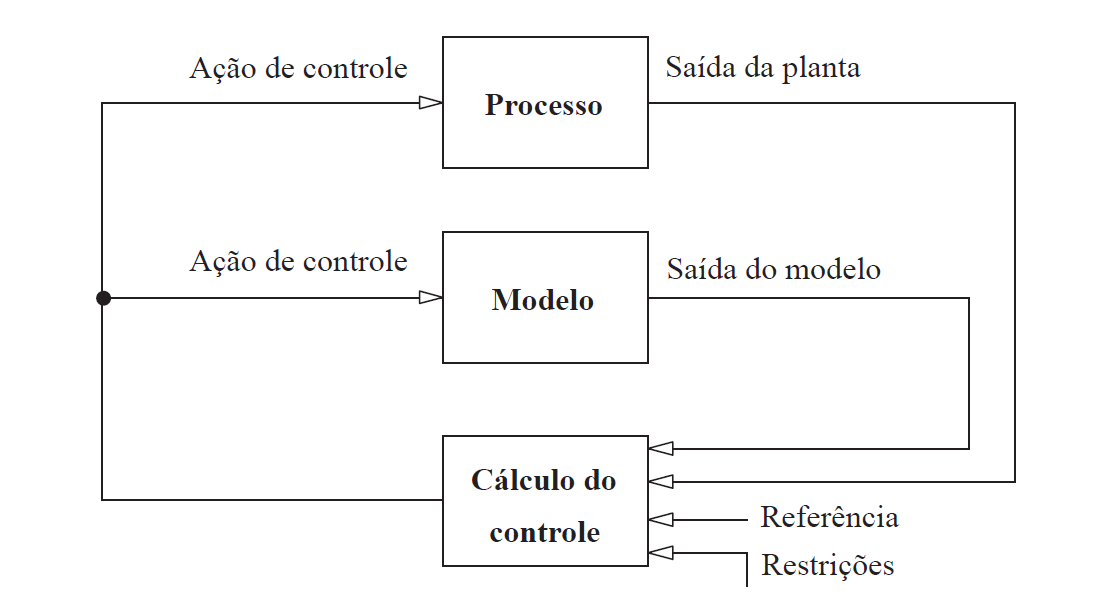
\includegraphics[scale=0.35]{figs/MPCbase.PNG}
%	   \caption{Algoritmo MPC}
%	   \label{label para referencia cruzada Figura}
%\end{figure}


% Lista de Item

%\begin{itemize}
%	\item item 1
%	\item item 2
%	\item item 3
%\end{itemize}

% Equação
%\begin{equation}
%	\label{label para referencia cruzada %equacoes}
%	y(t)=\sum_{i=1}^{\infty}h_i\Delta u(t-i)
%\end{equation}

% Equação em linha
%$\hat{y}(t+k\mid t)= \sum^\infty_{i=1} g_i %\Delta u(t+k-i\mid t)$

% Citação -  Criei o arquivo de bibliografia usando o jabref

%\cite{Camacho2007}

% Referencia Cruzada de Figura
%\ref{label para referencia cruzada Figura}

% Referencia Cruzada de Equação
%\ref{label para referencia cruzada equacoes}


% Tabelas

%\begin{table}[h]
%\begin{center}
%     \caption{Índices 1 para casos factíveis}
%     \begin{tabular}{| l | l | l | l |}
%     \hline Índice & LP Petro & LP 2 & %Diferença\\
%     \hline $SES_y$& 60.5406 & 60.5492 & %-0.0087\\
%     \hline $SES_u$& 1166.1464 & 1166.1464 & 2.36*$10^{-9}$ \\
%     \hline

%    \end{tabular}
%\label{table:indices1}
%\end{center}
%\end{table}
